\documentclass[a4paper,10pt]{report}
\usepackage[utf8]{inputenc}
\usepackage[T1]{fontenc}
\usepackage{graphicx}

% Title Page
\title{Algorithmes adaptatifs}
\author{Adrien DROGUET}


\begin{document}
\maketitle

%\begin{abstract}
%\end{abstract}

\chapter{Algorithmes génétiques}
\section{Variables d'exécution}
\begin{itemize}
  \item \textbf{pop\_size} : Taille de la population, par défaut 200.
  \item \textbf{numberOfIterations} : Nombre d'itérations de l'algorithme avant terminaison, par défaut 300.
  \item \textbf{k} : Nombre de flips à faire lors d'un k-flip, par défaut 3.
  \item \textbf{t} : Nombre d'individus d'un tournoi, par défaut 5.
\end{itemize}



\section{Algorithmes disponibles}
\subsection{Sélection}
Par défaut: \textit{tournament}.
\begin{itemize}
  \item \textbf{Best} : Choisit les deux meilleurs instances.
  \item \textbf{Random} : Choisit deux instances aléatoires.
  \item \textbf{Worst-Best} : Choisit la meilleure et la pire instance.
  \item \textbf{Tournament} : Sélectionne les deux meilleures instances d'une sous-population.
\end{itemize}


\subsection{Croisement}
Par défaut: \textit{cross point}
\begin{itemize}
  \item \textbf{Cross Point} : Coupe deux instances à un point aléatoire.
  \item \textbf{Cross Uniform} : Mélange le contenu de deux instances.
\end{itemize}


\subsection{Mutation}
Par défaut: \textit{Bit Flip}
\begin{itemize}
   \item \textbf{Bit Flip} : Chaque bit d'une instance a 1/n chances d'être inversé.
   \item \textbf{K Flip} : Inverse k bits d'une instance.
\end{itemize}


\subsection{Insertion}
Par défaut: \textit{Replace Worst}
\begin{itemize}
  \item \textbf{Compare with parents} : Compare et (potentiellement) remplace les parents des instances générées.
  \item \textbf{Age} : Remplace les plus vieilles instances d'abord.
  \item \textbf{Replace Worst} : Remplace les pires instances.
\end{itemize}


\pagebreak
\section{Tests et résultats}
Chaque graphique représente la moyenne de 10 lancement pour la configuration décrite.

\subsection{Configuration par défaut}
\begin{figure}[h]
  \begin{center}
    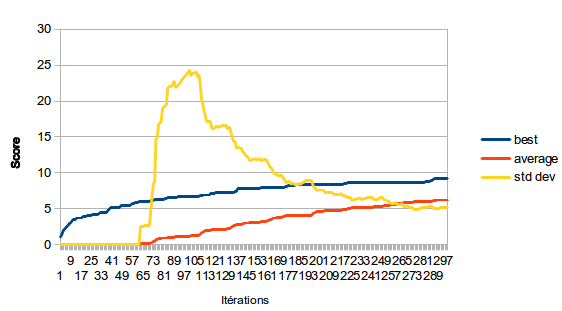
\includegraphics[width=320px]{images/graph-default.png}
  \end{center}
  \caption{tournament - cross point - bit-flip - replace worst}
\end{figure}

\subsection{Variation de sélection}
\subsubsection{Random}
\begin{figure}[h]
  \begin{center}
    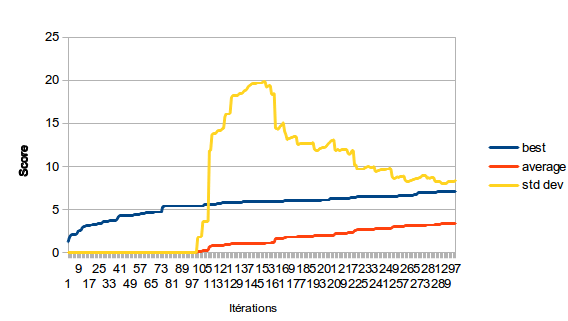
\includegraphics[width=320px]{images/graph-random.png}
  \end{center}
  \caption{random - cross point - bit-flip - replace worst}
\end{figure}

\subsection{Variation de croisement}
\subsubsection{Cross Uniform}
\begin{figure}[h]
  \begin{center}
    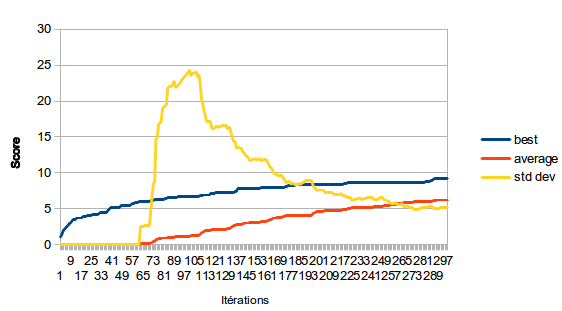
\includegraphics[width=320px]{images/graph-cross-uniform.png}
  \end{center}
  \caption{tournament - cross uniform - bit-flip - replace worst}
\end{figure}

\pagebreak
\subsection{Variation de mutation}
\subsubsection{3-Flip}
\begin{figure}[h]
  \begin{center}
    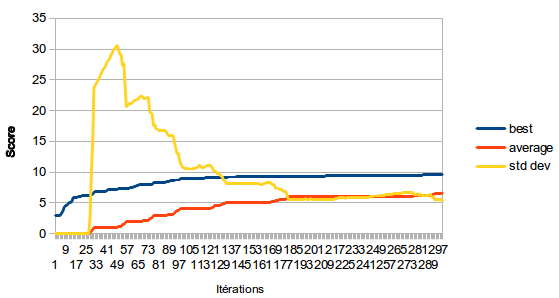
\includegraphics[width=320px]{images/graph-3-flip.png}
  \end{center}
  \caption{tournament - cross point - 3-flip - replace worst}
\end{figure}

\subsubsection{5-Flip}
\begin{figure}[h]
  \begin{center}
    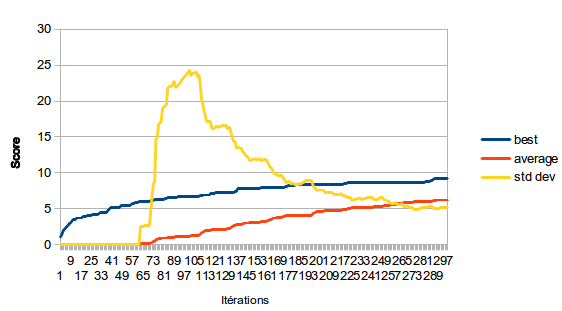
\includegraphics[width=320px]{images/graph-5-flip.png}
  \end{center}
  \caption{tournament - cross point - 5-flip - replace worst}
\end{figure}


\pagebreak
\subsection{Variation d'insertion}
\subsubsection{Age}
\begin{figure}[h]
  \begin{center}
    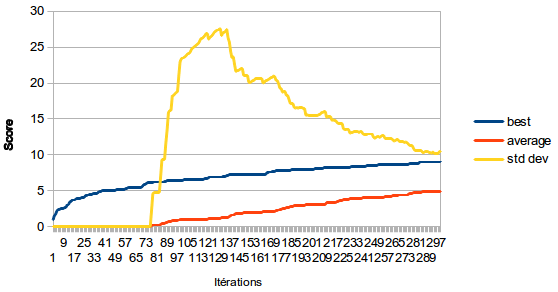
\includegraphics[width=320px]{images/graph-age.png}
  \end{center}
  \caption{tournament - cross point - bit-flip - age}
\end{figure}



\chapter{Algorithmes autonomes}
\section{Algorithmes considérés}
\subsection{}

\section{Tests et résultats}


\end{document}          
